\epi{"I am interested in this and hope to do something."}
{\textit{On adding complex numbers to Go}\\ \textsc{KEN THOMPSON}}

\noindent{}This is an introduction to the Go language from Google. Its aim
is to provide a guide to this new and innovative language. 

Its intended audience is people who are familiar with programming
and know multiple programming languages, be it C\cite{c}, C$^{++}$\cite{c++}, 
Java \cite{java}, Erlang\cite{erlang}, Scala\cite{scala} or
Haskell\cite{haskell}. This is \emph{not} a book which teaches you how to 
program, this is a book that just teaches you how to use Go.

As with
learning new things, the best way to do this is to discover it for
yourself by creating your own programs.
Each chapter includes a number of exercises (and answers)
to acquaint you with the language.
An exercise
is numbered as \textbf{Q$n$}, where $n$ is a number. After the
exercise number another number in parentheses displays the difficulty
of this particular assignment. This difficulty ranges from 0 to
50 \footnote{This is the same scale Donald Knuth uses.}, where
0 is easy and 50 is extremely difficult (such a problem is a unresolved
research problem). Then a short name is given, for easier reference.
For example
\begin{verse}
\textbf{Q1}. (4) A map function \ldots
\end{verse}
    
introduces a question numbered \textbf{Q1} of a level 4 difficulty, concerning a
\func{map()}-function. The answers are included after the exercises on a
new page, except for those pesky unresolved research problems.
The numbering and setup of the answers is identical to the
exercises, except that an answer starts with \textbf{A$n$}, where the
number $n$ corresponds with the number of the exercise.

Go is a young language, where 
features are still being added or even \emph{removed}. It 
may be possible that some text is outdated when you
read it. 
Some exercise answers may become incorrect as Go continues
to evolve.
We will do our best to keep this document up to 
date with respect to the latest Go release.
An effort has been made to create "future proof" code examples.
\noindent{}The following convention is used throughout this book:
\begin{itemize}
\item Normal text is typeset use the Droid Fonts;
\item Code is displayed in \prog{DejaVu Mono};
\item Keywords are displayed in \key{DejaVu Mono Bold};
\item Comments are displayed in \rem{DejaVu Mono Italic};
\item Extra remarks in the code \coderemark{Are displayed like this};
\item Longer remarks get a number -- \gocircle{1} -- with the explanation following;
\item Line numbers are printed on the right side;
\item Shell examples use a \pr{} as prompt;
\item An emphasised paragraph is indented and has a vertical bar on the
left.
\end{itemize}

\section{Official documentation}
There already is a substantial amount of documentation written about Go.
The Go Tutorial \cite{go_tutorial}, and the Effective Go
document \cite{effective_go}. The
website \url{http://golang.org/doc/} is a very good starting point
for reading up on Go\footnote{\url{http://golang.org/doc/} itself is served by 
a Go program called \prog{godoc}.}. Reading these documents is
certainly not required, but is recommended.

\section{Getting Go for Linux}
There are currently (2010) no packages for Go in any Linux
distribution. The route to install Go is thus slightly longer than
it could be. When Go stabilizes this situation will change probably. For
now, you need to retrieve the code from the mercurial archive and compile
Go yourself.
\begin{itemize}
\item First install Mercurial (to get the \prog{hg} command). In
Ubuntu/Debian/Fedora you must install the \prog{mercurial} package;

\item For building Go you also need the packages: \prog{bison},
\prog{gcc}, \prog{libc6-dev}, \prog{ed}, \prog{gawk} and \prog{make};

\item Then retrieve the Go source code:
\begin{display}
\pr export GOROOT=~/go	\rem{\# set the GOROOT environment variable}
\pr hg clone -r release https://go.googlecode.com/hg/ $GOROOT 
\end{display}

\item Set your PATH to find the Go binaries:
\begin{display}
\pr export PATH=$GOROOT/bin:$PATH
\end{display}

\item Compile Go
\begin{display}
\pr cd $GOROOT/src
\pr ./all.bash
\end{display}
\end{itemize}
If all goes well, you should now have Go installed on your system and
you can start playing.

\section{Online documentation}
Go comes with its own documentation in the form of a Go program called
\prog{godoc}. 
You can use it yourself to look
in the online documentation. For
instance, suppose we want to know more about the package \package{hash}.
We would then give the command \prog{godoc hash}.
How to read this and how you can create your own package documentation
is explained in chapter \ref{chap:packages}.

\section{Origins}
Go has it origins in Plan 9 \cite{plan9}. Plan 9 is (or was 
supposed to be) the successor of Unix. As you know one of the
core ideas of Unix is "everything is a file", so the \func{read()} and
\func{write()} calls work as well on normal files as they do on I/O
devices. However for some devices this has never happened, notably
network and video devices. In Plan 9 this "everything is a file"--idea
is taken to the next level and truly everything is presented to the 
user as a file, including networking and video devices. This has nothing
to do with Go per se, but Plan 9 included a language called Limbo
\cite{limbo}. Quoting from the Limbo paper:
\begin{quote}
Limbo is a programming language intended for applications running
distributed systems on small computers. It supports modular programming,
strong type checking at compile- and run-time, \emph{inter process
communication over typed channels}, automatic \emph{garbage collection}, and
simple abstract data types. It is designed for safe execution even on
small machines without hardware memory protection.
\end{quote}
That sounds a lot like Go, and one could say Go is a reimplementation of
Limbo on Unix--like systems like Linux. One feature of Limbo that is
also included in Go is the excellent support for cross compiling.

Another feature Go inherited from Limbo is channels (see chapter
\ref{chap:channels}). Again from the documentation.
\begin{quote}
[A channel] is a communication mechanism capable of sending and receiving objects of
the specified type to another agent in the system. Channels may be used
to communicate between local processes; using library procedures, they
may be connected to named destinations. In either case send and receive
operations may be directed to them.
\end{quote}
The channels in Go are easier to use than those in Limbo.
If we dig even deeper in the history of Go we also find references
to "Newsqueak" \cite{newsqueak}, which pioneered the use of 
channel communication in a C--like language. Channel
communication isn't unique to these languages, a big non--C--like
language which also uses them is Erlang \cite{erlang}.

\begin{figure}[H]
\caption{Chronology of Go}
\label{fig:chrono-of-go}
\begin{center}
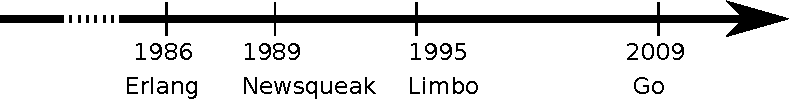
\includegraphics[scale=0.65]{fig/go-history.pdf}
\end{center}
\end{figure}

The whole of idea of using channels to communicate with other processes
is called Communicating Sequential Processes (CSP) and was conceived
by C. A. R. Hoare \cite{hoare}, who incidentally is the same man that
invented QuickSort \cite{Quicksort}.

\begin{lbar}
Go is the first C--like language that is widely available,
runs on many
different platforms and makes concurrency easy (or easier).
Becoming proficient in a new language means doing your exercises,
reading about it helps, but getting down to the little details when 
programming your self is even better.
\end{lbar}

\section{Exercises}
\begin{Exercise}[title={文档},difficulty=1]
\label{ex:doc}
\Question
Go 的文档可以通过~\prog{go doc} 程序阅读,它包含在~Go 的发布包中。

\prog{go doc hash} 给出了~\package{hash} 包的信息:
\vskip\baselineskip
\begin{display}
\pr \user{go doc hash}
PACKAGE

package hash

...
...
...

SUBDIRECTORIES

        adler32
        crc32
        crc64
        fnv

\end{display}
\vskip\baselineskip
哪个~\prog{go doc} 的命令可以显示~\package{hash} 包中的~\package{fnv} 文档?

\end{Exercise}

\begin{Answer}
\Question
\package{fnv} 包在~\package{hash} 的\emph{子目录}中,所以只需要 
\quad \texttt{go doc hash/fnv} 即可。


所有的内建函数同样可以通过~\prog{godoc} 程序访问:\prog{go doc builtin}。
\end{Answer}


\cleardoublepage
\section{Answers}
\shipoutAnswer
